\chapter{Persistência em arquivos}
	
Aplicações precisam de algum mecanismo de persistência de dados, pois informações armazenadas na memória são perdidas sempre que a aplicação é encerrada. A forma mais simples de fazer isso em Java é salvar os dados em arquivos. As operações de leitura e escrita de dados em arquivos são feitas através das bibliotecas de entrada e saída do Java (ou bibliotecas I/O – Input/Output). A Figura~\ref{fig:file-esquema} mostra o esquema geral da biblioteca de entrada e saída que será usada neste capítulo. O programa em Java comunica-se com as classes \code{FileReader} e \code{FileWriter} para as operações de leitura e gravação de dados no arquivo.

\begin{figure}[h]
	\centering
	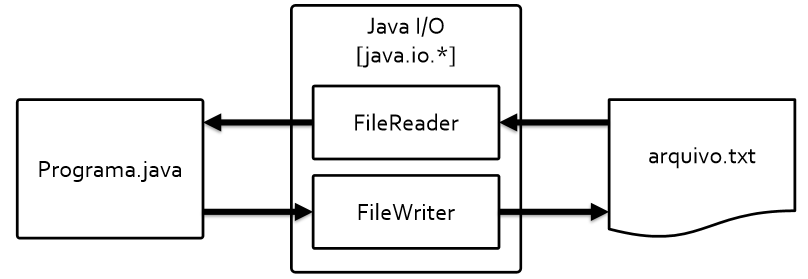
\includegraphics[width=0.4\textheight]{img/file-esquema}
	\caption{Esquema de classes para persistência em arquivos}
	\label{fig:file-esquema}
\end{figure}

\section{Operação de escrita}

A classe \code{FileWriter} fornece os métodos necessários para a escrita de dados em arquivos. Na sua criação, é passado o nome do arquivo e o argumento \code{append}. Se verdadeiro, caso existam informações no arquivo, elas são mantidas e os novos dados são inseridos no final do arquivo. Se falso, caso existam informações no arquivo, elas são apagadas e os novos dados são inseridos no seu lugar.

O trecho de código abaixo mostra o uso da classe \code{FileWriter} para escrita de dados. O método \code{write} recebe como parâmetro o valor e o escreve no arquivo vinculado ao \code{writer} (neste exemplos, \texttt{pessoas.txt}). Repare que é necessário fechar o \code{writer} após o uso, bem como circundar o código com instruções \code{try-catch} para tratar o disparo de exceções no acesso ao arquivo em disco.

\begin{minted}{java}
try {
	FileWriter writer = new FileWriter("pessoas.txt", true);
	writer.write("Este texto será inserido no arquivo");
	writer.write("\n");
	writer.close();
} catch (IOException ex) {
	Logger.getLogger(
		PersistenciaArquivos.class.getName()).log(Level.SEVERE, null, ex);
}
\end{minted}

\section{Operação de leitura}

A classe \code{FileReader} fornece métodos para abertura de arquivos e leitura dos seus dados. Porém, seus métodos permitem apenas a leitura de caracteres. Para ler os dados por linha, utilizaremos um objeto da classe \code{BufferedReader}. Na criação, instanciamos um novo \code{FileReader} passando o nome do arquivo.

O trecho de código mostra a implementação do método de leitura de dados usando as classes supracitadas. O método \code{readLine} faz a leitura de toda a linha e passa para a próxima. Após ler a última linha do arquivo, o método devolve \code{null}. Por isso, enquanto a linha lida for diferente de nulo, a linha é impressa em tela. Após o término, o \code{reader} é fechado. Assim como os métodos de escrita, o código deve ser circundado com as instruções \code{try-catch}.

\begin{minted}{java}
try {
	BufferedReader reader = new BufferedReader(new FileReader("pessoas.txt"));
	String linha;
	while((linha = reader.readLine()) != null) {
		System.out.println(linha);
	}
	reader.close();
} catch (FileNotFoundException ex) {} catch (IOException ex) {}
\end{minted}


\section{Exemplo -- Cadastro de Pessoas}

Considere um sistema para cadastro de pessoas com persistência dos dados em arquivos texto. O sistema deve fornecer as operações de cadastro, exclusão, consulta de uma pessoa pelo seu nome e consulta de todas as pessoas cadastradas.

\subsection{Entidade Pessoa}

O trecho de código abaixo mostra a classe \code{Pessoa}, que define a entidade que será cadastrada e persistida. Repare no método \code{toWriteString} (linhas 8 a 10), que retorna o texto que será usado para armazenar a pessoa no arquivo, com cada atributo separado pelo caracter \texttt{';'}. O método \code{toString}, por sua vez, retorna o texto que deve ser usado para apresentar o objeto em tela.

\begin{minted}{java}
public class Pessoa {
	private String nome;
	private int idade;
	private char sexo;

	//Métodos construtores omitidos

	public String toWriteString() {
		return nome + ";" + idade + ";" + sexo;
	}

	public String toString() {
		String genero;
		if(sexo == 'M') genero = "masculino";
		else genero = "feminino";
		return nome + ", possui " + idade + " anos de idade e é do sexo " + genero + ".";
	}

	//Métodos acessores omitidos
}
\end{minted}

\subsection{Classe para persistência de dados}

O trecho de código abaixo mostra a classe \code{PersistenciaArquivos}, cuja responsabilidade é fornecer métodos para as operações desejadas (cadastro, exclusão e consulta de pessoas). O método \code{inserir} armazena uma pessoa no arquivo. O método \code{ler} recupera uma pessoa do arquivo pelo seu nome, recebido como argumento. O método \code{lerTodasPessoas} devolve uma lista com todas as pessoas armazenadas no arquivo. O método \code{excluir} remove uma pessoa do arquivo pelo seu nome, recebido como argumento.

\begin{minted}{java}
public class PersistenciaArquivos {
	public static void excluir(String nome) {
		//...
	}

	public static List<Pessoa> lerTodasPessoas() {
		//...
	}

	public static Pessoa ler(String nome) {
		//...
	}

	public static void inserir(Pessoa p){
		//...
	}
}
\end{minted}

\subsection{Escrita de uma pessoa}

O método \code{inserir} recebe um objeto da classe \code{Pessoa} e o armazena no arquivo. Seu código é apresentado abaixo. Neste processo, o método armazena no arquivo o conteúdo retornado pelo método \code{toStringFile}. Cada pessoa é escrita em uma linha, portanto ao final de cada pessoa é armazenada uma quebra de linha (\code{\textbackslash n}).

\begin{minted}{java}
public static void inserir(Pessoa p){
	try {
		FileWriter writer = new FileWriter("pessoas.txt", true);
		writer.write(p.toWriteString());
		writer.write("\n");
		writer.close();
	} catch (IOException ex) {
		Logger.getLogger(PersistenciaArquivos.class.getName()).log(
			Level.SEVERE, null, ex);
	}
}
\end{minted}

\subsection{Leitura de uma pessoa}

O código abaixo mostra a implementação do método \code{ler}, que recebe o nome de uma pessoa (\code{String}) e retorna um objeto da classe \code{Pessoa} com a referência buscada, caso encontrado. Caso contrário, o método retorna \code{null}. O arquivo é lido linha por linha, ou seja, enquanto o retorno do método \code{readLine} for diferente de \code{null} (linha 5). Cada linha é dividida pelo caracter separador (\texttt{';'}), de modo a obter o valor de cada atributo da pessoa armazenada no arquivo. Esta operação é feita pelo método \code{split} (linha 6 -- detalhado abaixo). Caso o nome da pessoa seja igual ao nome buscado, a pessoa é recuperada (linha 7). Nas linhas 8 a 13 o objeto \code{Pessoa} é criado e seus atributos são recuperados, para então retorná-lo.

\begin{minted}{java}
public static Pessoa ler(String nome) {
	try {
		BufferedReader reader = new BufferedReader(new FileReader("pessoas.txt"));
		String linha;
		while((linha = reader.readLine()) != null) {
			String[] conteudo = linha.split(";");
			if(conteudo[0].equals(nome)) {
				Pessoa p = new Pessoa();
				p.setNome(conteudo[0]); //nome na [0]
				p.setIdade(Integer.parseInt(conteudo[1])); //idade na [1]
				p.setSexo(conteudo[2].charAt(0)); //sexo [2]
				reader.close();
				return p;
			}
		}
		reader.close();
	} catch (FileNotFoundException ex) {} catch (IOException ex) {}
	return null;
}
\end{minted}

O método \code{split} divide a \code{String} conforme o caracter recebido (no exemplo, é usado o caracter \texttt{';'}). Ele separa cada valor e adiciona em uma posição de um vetor de String, retornando-o. O código abaixo exemplifica o uso do método \code{split}.

\begin{minted}{java}
String texto = "Este texto;está separado;para posterior;recuperação!";
String[] conteudo = texto.split(";");
\end{minted}

\begin{minipage}{\textwidth}
	\textbf{\texttt{Resultado:}}\\
	\texttt{\code{conteudo[0]}    ``Este texto''}\\
	\texttt{\code{conteudo[1]}    ``está separado''}\\
	\texttt{\code{conteudo[2]}    ``para posterior''}\\
	\texttt{\code{conteudo[3]}    ``recuperação!''}\\
\end{minipage}


\subsection{Leitura de todas as pessoas}

O trecho de código a seguir mostra a implementação do método \code{lerTodasPessoas}, que faz a leitura de todos os registros de pessoas armazenados no arquivo, retornando uma lista de objetos da classe \code{Pessoa}. A leitura é igual à de uma pessoa, mas todas as linhas são lidas, atribuídas ao objeto Pessoa e incluídos na lista, que é devolvida ao final do método.

\begin{minted}{java}
public static List<Pessoa> lerTodasPessoas() {
	List<Pessoa> listaPessoas = new ArrayList<Pessoa>();
	try {
		BufferedReader reader = new BufferedReader(new FileReader("pessoas.txt"));
		String linha;
		while((linha = reader.readLine()) != null) {
			String[] conteudo = linha.split(";");
			Pessoa p = new Pessoa();
			p.setNome(conteudo[0]);
			p.setIdade(Integer.parseInt(conteudo[1]));
			p.setSexo(conteudo[2].charAt(0));
			listaPessoas.add(p);
		}
		reader.close();
	} catch (FileNotFoundException ex) {} catch (IOException ex) {}
	return listaPessoas;
}
\end{minted}

\subsection{Exclusão de uma pessoa}

Como não existe um método para excluir uma linha única de um arquivo, a estratégia de exclusão consiste em ler todos os dados, apagar todo o arquivo e reescrever todos os registros novamente, exceto aquele que deve ser excluído. O trecho de código abaixo mostra a implementação do método \code{excluir}. Repare que o método carrega uma lista com todas as pessoas (linha 2) e a percorre. Apenas os dados da pessoa buscada não são inseridos na \code{String} a ser regravada (linhas 6 e 7). Após lidas todas as pessoas, o arquivo é aberto com modo \code{append = false}, que apaga todos os registros previamente armazenados, para então gravar os novos dados.

\begin{minted}{java}
public static void excluir(String nome) {
	List<Pessoa> todasPessoas = lerTodasPessoas();
	String conteudo = "";

	for(Pessoa p : todasPessoas) {
		if(!p.getNome().equals(nome))
			conteudo += p.toWriteString() + "\n";
	}

	try {
		FileWriter writer = new FileWriter("pessoas.txt", false);
		writer.write(conteudo);
		writer.close();
	} catch (IOException ex) {
		Logger.getLogger(PersistenciaArquivos.class.getName()).log(
			Level.SEVERE, null, ex);
	}
}
\end{minted}

\textbf{OBS:} uma estratégia similar pode ser adotada na edição de dados, onde todos os registros são reescritos, atualizando os atributos do registro buscado.